% translate_docs: ./cars/E-GMP_gen1/Ioniq6/head_unit_preconditioning_kit_Ioniq6_install.tex @ 1310963db16097b8980375704a3fc258a6de4b75
\documentclass[superscriptaddress,onecolumn,floatfix]{revtex4-2}

\usepackage{graphicx}
\usepackage{epsfig}
\usepackage{color}
\usepackage{amssymb}
\usepackage{amsmath}
\usepackage{array}
\usepackage[loose]{units}
\usepackage{hyperref}
\usepackage{cleveref}
\usepackage{braket}
\usepackage[caption=false]{subfig}
\usepackage[german]{babel}
\usepackage{letltxmacro}

\pdfcompresslevel=9

\LetLtxMacro{\ORIGselectlanguage}{\selectlanguage}
\makeatletter
\DeclareRobustCommand{\selectlanguage}[1]{%
    \@ifundefined{alias@\string#1}
      {\ORIGselectlanguage{#1}}
      {\begingroup\edef\x{\endgroup
         \noexpand\ORIGselectlanguage{\@nameuse{alias@#1}}}\x}%
}
\newcommand{\definelanguagealias}[2]{%
  \@namedef{alias@#1}{#2}%
}
\makeatother

\definelanguagealias{de}{german}


\begin{document}
\selectlanguage{de}

\begin{abstract}
Diese Anleitung führt Sie durch die notwendigen Schritte zur Installation des Vorkonditionierungskits für das Autoradio in Ihrem Ioniq 6 (Modelljahre 2023–2025). 
\begin{description}
  \item[Schritt 1: 12V-Anschluss trennen] 
  \item[Schritt 2: Zuschneiden]
  \item[Schritt 3: Kabelbaumanschluss] 
  \item[Schritt 4: OBD-Halterung] 
  \item[Schritt 4.5: WiCAN-Plug-in] 
\end{description}
\end{abstract}
\title{Installationsanleitung für das Vorkonditionierungsset: Ioniq 6}
\author{Ioniq Guy}
\author{Electroniq Buttons Boutique}
\email{support@electroniqbuttons.com}
% \affiliation{\GOE}
% \author{Benjamin J. McMorran}
% \email{mcmorran@uoregon.edu}
% \affiliation{\UO}
\date{\today}

\maketitle

\begin{figure}[h]
  \subfloat[]{\label{subfig:overview:harness}
  \includegraphics[height=1.95in]{../../../harnesses/head_unit_MITM/photos/whole_harness.jpg} } \\
  % \subfloat[]{\label{subfig:overview:trim}
  % \includegraphics[width=6in]{photos/overview_labeled.jpg} }
   \caption{(a) Mann-in-der-Mitte-Gurtzeug. \label{fig:overview}}
\end{figure}

\section{Einführung}
  Diese Anleitung dient dazu, die schrittweise Installation des Vorkonditionierungskits für das Steuergerät bzw. des in Abbildung 1 dargestellten Kabelbaums für die Steuereinheit (Man-in-the-Middle-Kabelbaum) zu veranschaulichen. \ref{subfig:overview:harness}Im Abschnitt \ref{sect:1}In Abschnitt 1 beschreiben wir das Entfernen der Verkleidung, um Zugang zum Hauptgerät zu erhalten. \ref{sect:2}In Abschnitt 1 beschreiben wir den Vorgang des Anschließens des Kabelbaums. \ref{sect:3}Wir zeigen den Anschluss des OBD-Anschlusses und wie man den Mikrocontroller einsteckt. 

Erforderliche Werkzeuge:
\begin{enumerate}
  \item 10-mm-Steckschlüssel oder verstellbarer Schraubenschlüssel für 12-V-Batterie (nicht im Lieferumfang enthalten).
  \item Werkzeuge zum Entfernen der Zierleisten (bei Auswahl enthalten)
\end{enumerate}

Kit-Komponenten:
\begin{enumerate}
  \item Kabelbaum für das Hauptgerät
  \item WiCAN
  \item 70-mm-OBD-Halterung
  \item 70 mm doppelseitiges Klebeband (zwei Stücke zur Sicherheit enthalten)
  \item 4 Kabelbinder
\end{enumerate}

\section{Schritt 1: Den Minuspol der 12-V-Batterie abklemmen.} \label{sect:0}
Trennen Sie immer zuerst die 12-V-Batterie, bevor Sie irgendwelche elektrischen Steckverbinder entfernen! Das Entfernen eines stromführenden Steckers kann eine Entladung verursachen und einen Stecker oder das Steuergerät Ihres Autos zerstören.

Schritt-für-Schritt-Anleitung:
\begin{enumerate}
  \item Motorhaube öffnen % (Figure \ref{subfig:12V:hood})
  \item Öffnen Sie den Frunk (Abbildung \ref{subfig:12V:frunk})
  \item Entfernen Sie die Abdeckung für die 12-V-V-Anlage. % (Figure \ref{subfig:12V:panel})
  \item Die Mutter auf der Minusseite mit einer 10-mm-Nuss lösen. % (Figure \ref{subfig:12V:nut})
  \item Minuspol entfernen % (Figure \ref{subfig:12V:terminal})
\end{enumerate}

\begin{figure}[h]
  % \subfloat[]{\label{subfig:12V:hood}
  % \includegraphics[height=1.5in]{photos/open_hood.jpg} } 
  % \subfloat[]{\label{subfig:12V:panel}
  % \includegraphics[height=1.5in]{photos/remove_panel.jpg} }  \\
  % \subfloat[]{\label{subfig:12V:nut}
  % \includegraphics[height=1.5in]{photos/loosen_nut.jpg} } 
  % \subfloat[]{\label{subfig:12V:terminal}
  % \includegraphics[height=1.5in]{photos/disconnect_terminal.jpg} } 
  \subfloat[]{\label{subfig:12V:frunk}
  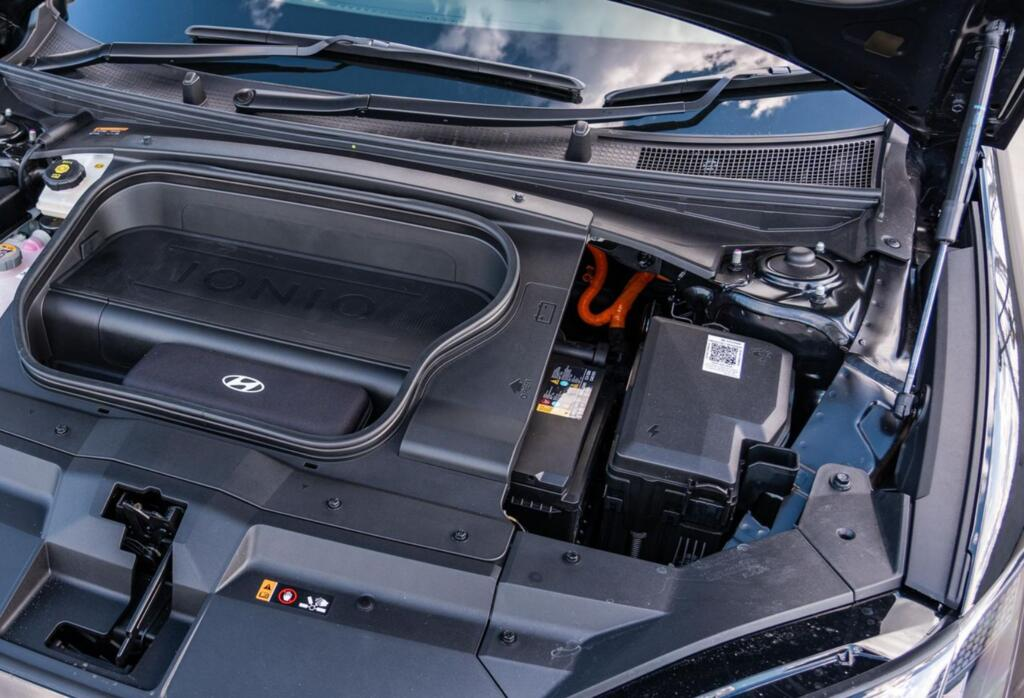
\includegraphics[height=1.5in]{photos/frunk.jpg} } 
  \caption{(a) Öffnen Sie den vorderen Kofferraum. \label{fig:12V}}
   % \caption{(a) Open the hood. (b) Remove panel covering 12V. (c) Loosen nut on negative terminal. (d) Remove negative terminal. \label{fig:12V}}
\end{figure}

\section{Schritt 2: Zuschneiden} \label{sect:1}
Das Ziel ist es, an den eigentlichen Schatz zu gelangen: das Hauptgerät. Es befindet sich hinter einer einzelnen Verkleidung, der sogenannten Crashpad-Unterabdeckung, die in Abbildung 1 mit einem X markiert ist. \ref{fig:step1}.
\begin{figure}[h]
  \subfloat[]{\label{subfig:step1:X}
  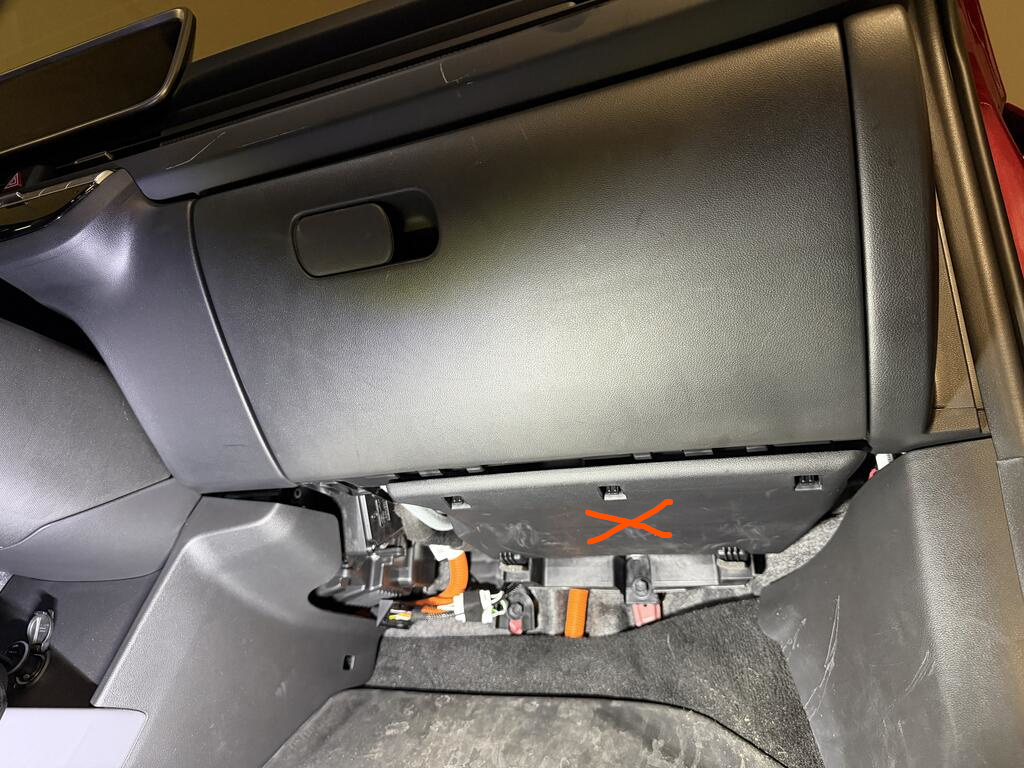
\includegraphics[height=2.95in]{photos/x_marks_HU.jpg} } 
   \caption{Das X markiert das Hauptgerät. \label{fig:step1}}
\end{figure}

Schritt-für-Schritt-Anleitung:
\begin{enumerate}
  \item Entfernen Sie das Crashpad unter der Abdeckung (Abbildung \ref{subfig:trim:crash_pad_under_cover}): 
    \begin{enumerate}
      \item Verwenden Sie ein Werkzeug zum Entfernen von Verkleidungen, um vorsichtig einen der drei Clips freizulegen (Abbildung \ref{subfig:trim:open})
      \item Drücken Sie auf die Lasche am Clip, die in Abbildung 1 mit Corbins Daumen markiert ist. \ref{subfig:trim:open}um den Clip zu veröffentlichen
    \end{enumerate}
  \item Entfernen Sie die Schrauben, mit denen die Kopfeinheit befestigt ist (Abbildung \ref{subfig:trim:HU_screws})
\end{enumerate}

\begin{figure}[h]
  \subfloat[]{\label{subfig:trim:crash_pad_under_cover}
  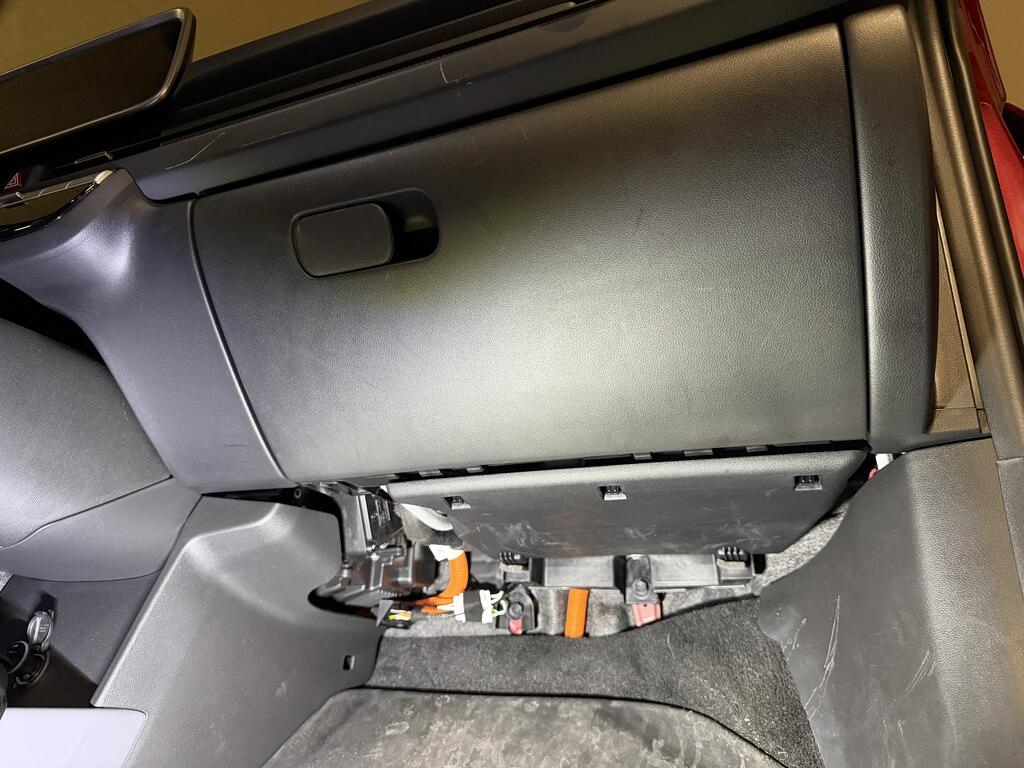
\includegraphics[height=1.5in]{photos/harness_installed_1.jpg} } 
  \subfloat[]{\label{subfig:trim:open}
  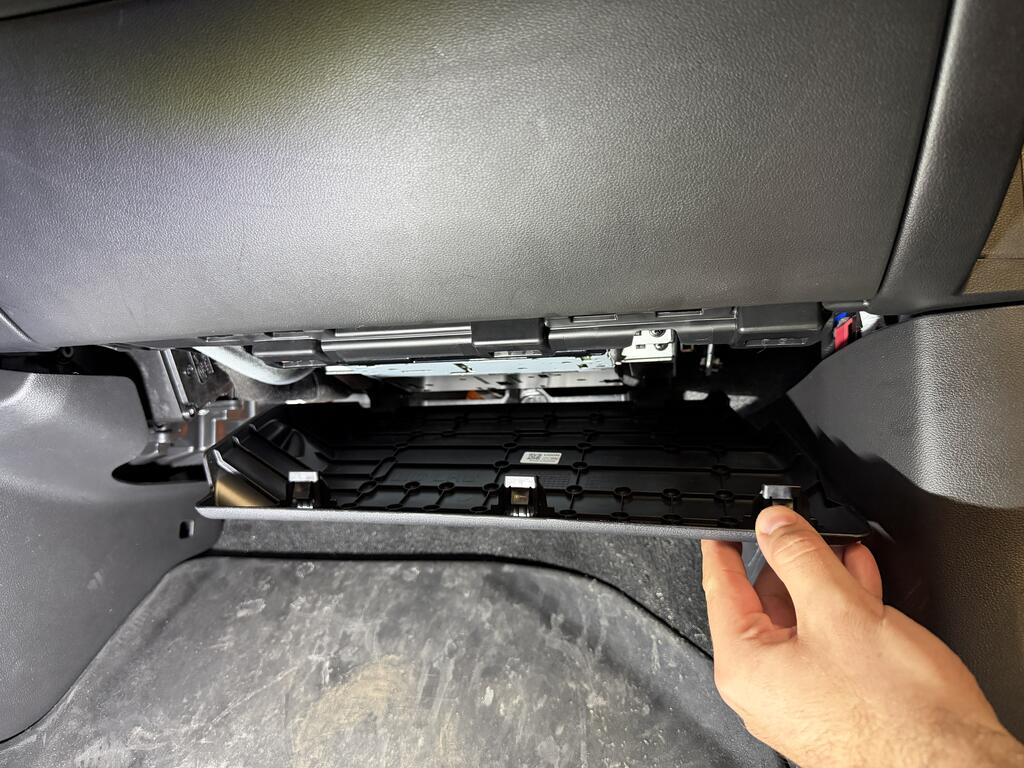
\includegraphics[height=1.5in]{photos/panel_open.jpg} } 
  \subfloat[]{\label{subfig:trim:HU}
  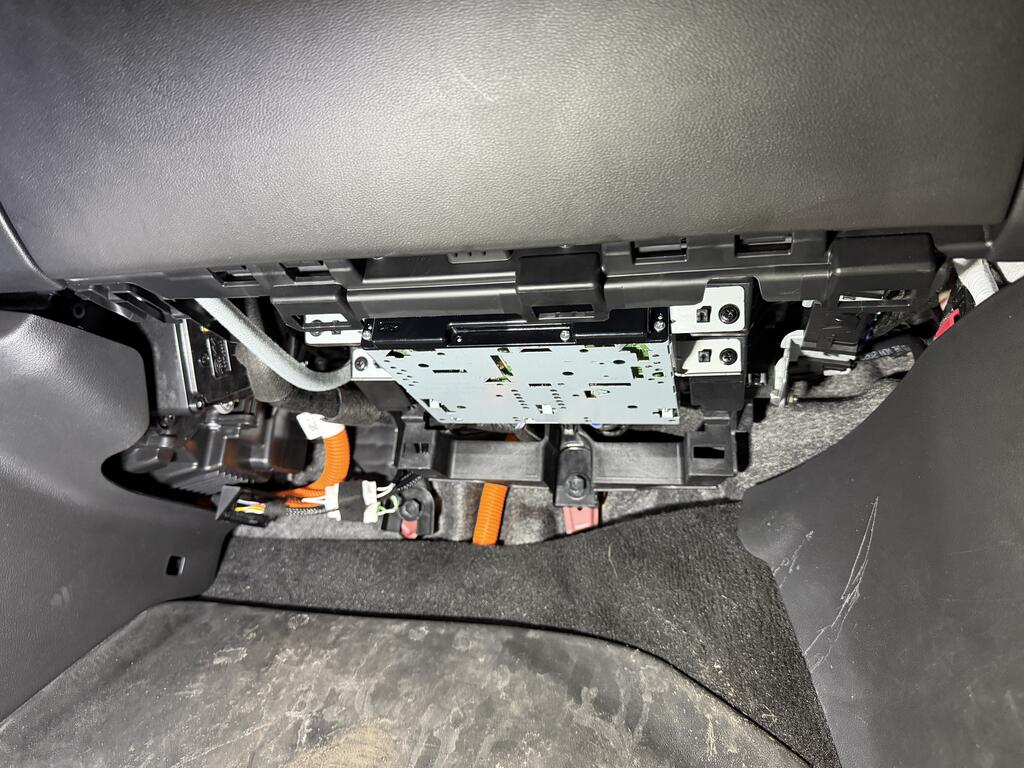
\includegraphics[height=1.5in]{photos/HU_exposed.jpg} } 
  \subfloat[]{\label{subfig:trim:HU_screws}
  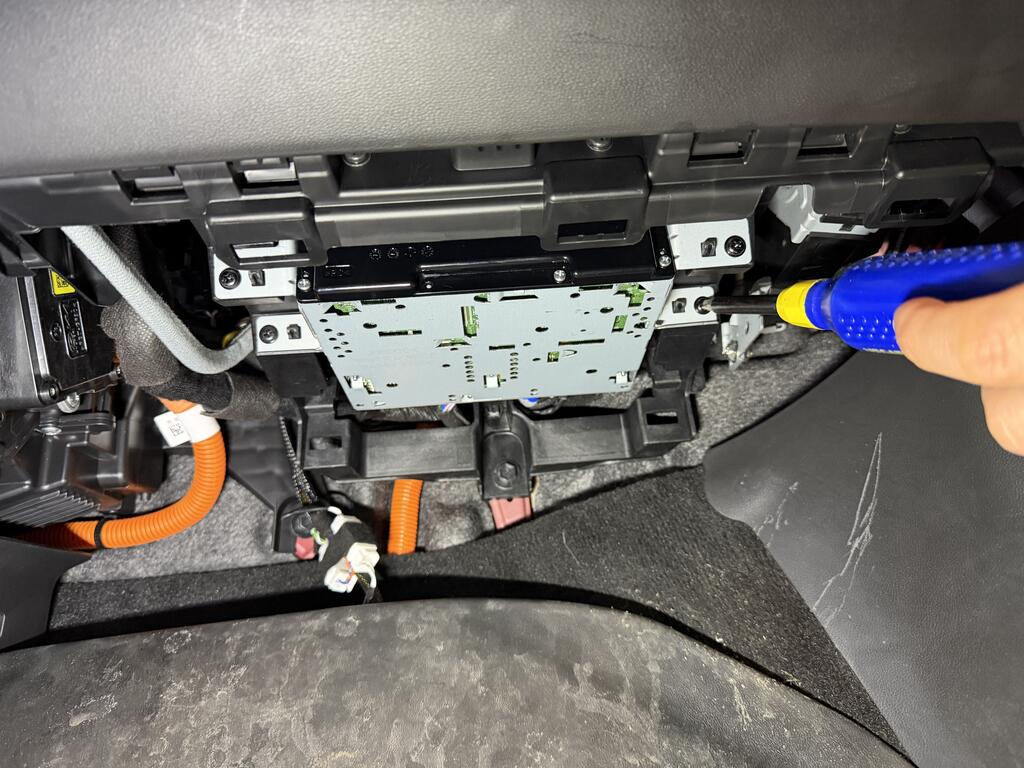
\includegraphics[height=1.5in]{photos/reinstalling_HU.jpg} } 
   \caption{(a) Sturzpolster unter der Abdeckung. (b) Entfernen des Sturzpolsters unter der Abdeckung. (c) Freiliegendes Hauptgerät. (d) Entfernen der Schrauben, mit denen das Hauptgerät befestigt ist. \label{fig:trim}}
\end{figure}


\section{Schritt 3: Kabelbaumanschluss} \label{sect:2}
Dieser Schritt umfasst den Einbau des Kabelbaums in das Hauptgerät. 

Schritt-für-Schritt-Anleitung:
\begin{enumerate}
  \item Identifizieren Sie den originalen grauen weiblichen Stecker der Steuereinheit (Abbildung \ref{subfig:harness:headunit_oe_connectors})
  \item Entfernen Sie es, indem Sie den Clip zusammendrücken und nach unten ziehen. 
  \item Stecken Sie den zuvor entfernten weiblichen Stecker in die männliche Seite des Kabelbaums (Abbildung \ref{subfig:harness:harness_male_in})
  \item Stecken Sie die weibliche Seite des Kabelbaums in die Kopfeinheit (Abbildung \ref{subfig:harness:harness_in})
\end{enumerate}

\begin{figure}[h]
  \subfloat[]{\label{subfig:harness:female}
  \includegraphics[height=1.5in,angle=0]{../../../harnesses/head_unit_MITM/photos/labeled_connectors_MITM_harness.jpg} } 
  \subfloat[]{\label{subfig:harness:male}
  \includegraphics[height=1.5in,angle=0]{../Ioniq5/photos/male_harness_end.jpg} }  \\
  \subfloat[]{\label{subfig:harness:headunit_oe_connectors}
  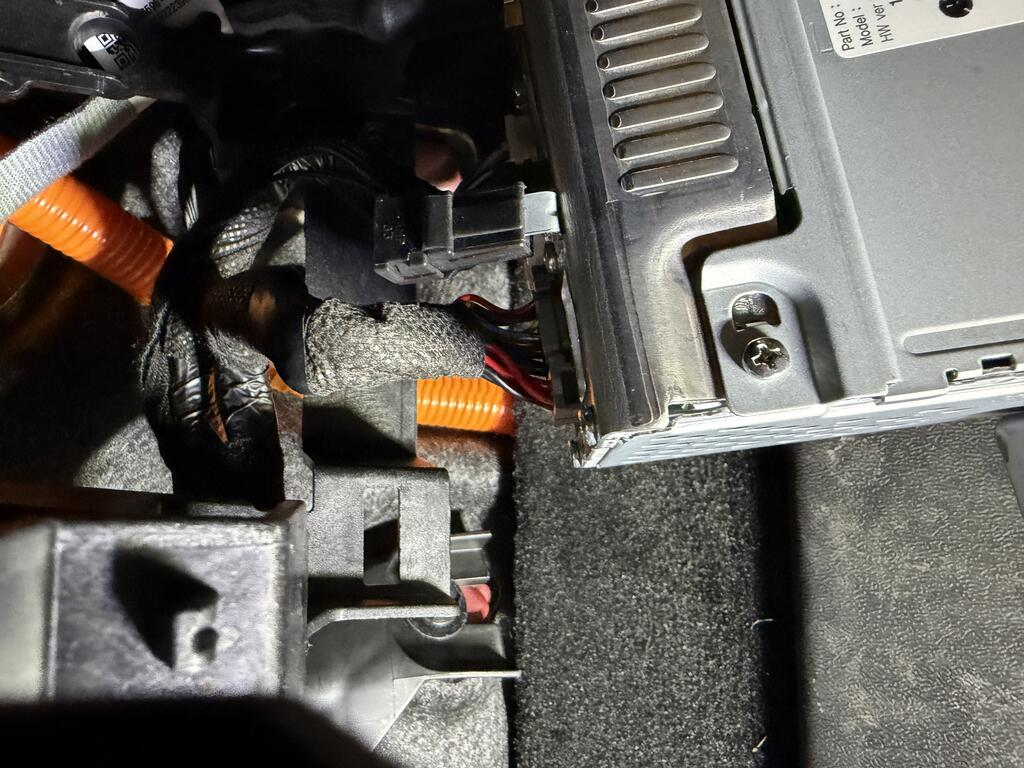
\includegraphics[height=1.5in,angle=0]{photos/HU_dangling_clip_detached.jpg} } 
  \subfloat[]{\label{subfig:harness:harness_male_in}
  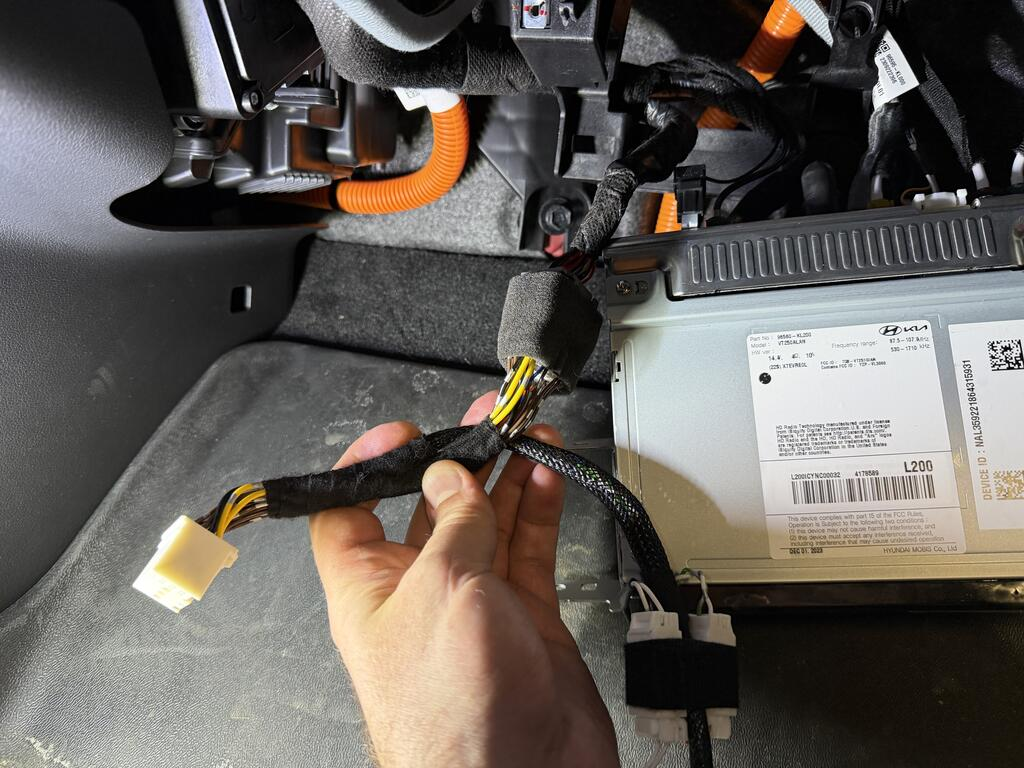
\includegraphics[height=1.5in,angle=0]{photos/harness_installing_3.jpg} } 
  \subfloat[]{\label{subfig:harness:harness_in}
  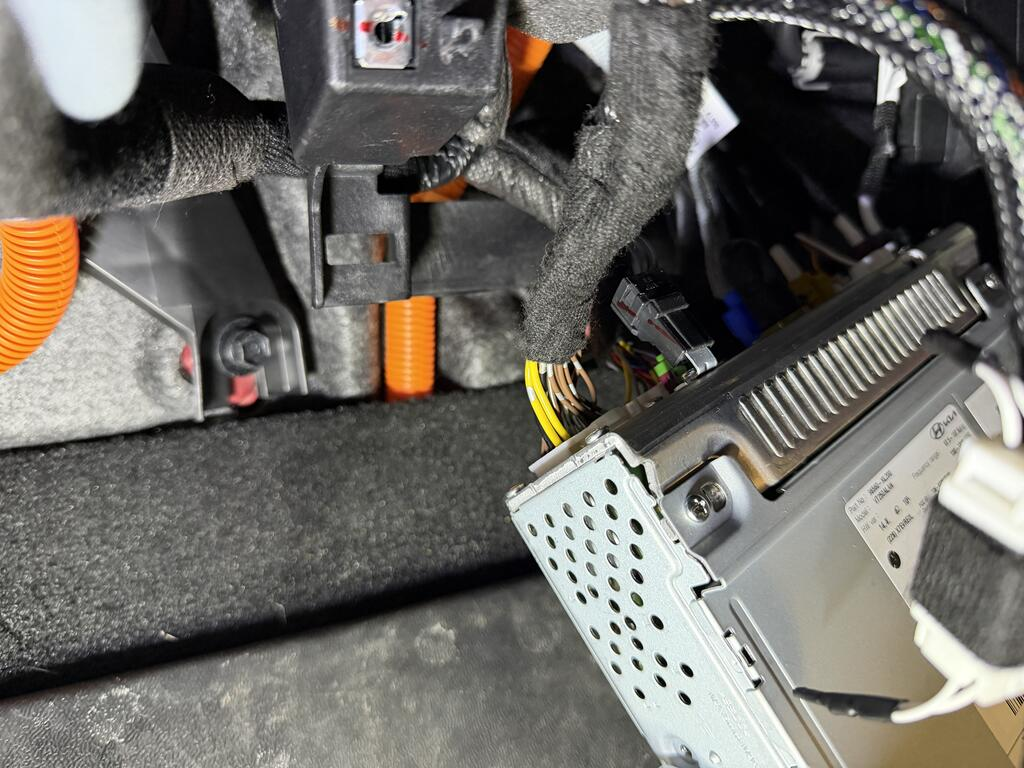
\includegraphics[height=1.5in,angle=0]{photos/HU_dangling_clip_detached_2.jpg} }  
   \caption{(a) Beschriftetes Foto mit weiblichem Kabelbaumstecker. (b) Männlicher Kabelbaumstecker. (c) Autoradio mit angeschlossenen Originalsteckern. (d) Weiblicher Stecker (grau) aus dem Autoradio entfernt. (e) Im Autoradio installierter Kabelbaum. \label{fig:harness}}
\end{figure}
\section{Schritt 4: OBD-Halterung} \label{sect:3}
In diesem Schritt montieren wir das OBD-Ende des Kabelbaums sicher und schließen den WiCAN an. 

Schritt-für-Schritt-Anleitung:
\begin{enumerate}
  \item Gewinde OBD Ende über der Halterung der Head Unit (Abbildung \ref{subfig:obd:thread_obd})
  \item Haupteinheit wieder einbauen. (Abbildung \ref{subfig:trim:HU_screws})
  \item Stecken Sie die OBD-Buchse in die mitgelieferte Halterung, falls diese noch nicht montiert ist.
  \item Verwenden Sie doppelseitiges Klebeband, um die Halterung an einer flachen Verkleidungsfläche zu befestigen.
  \item Verwenden Sie Kabelbinder, um den Kabelbaum an anderen Kabeln und Befestigungspunkten zu befestigen. 
  \item Halten Sie die Halterung fest und stecken Sie WiCAN ein (Abbildung \ref{subfig:obd:wican})
\end{enumerate}

\begin{figure}[h]
  \subfloat[]{\label{subfig:obd:thread_obd}
  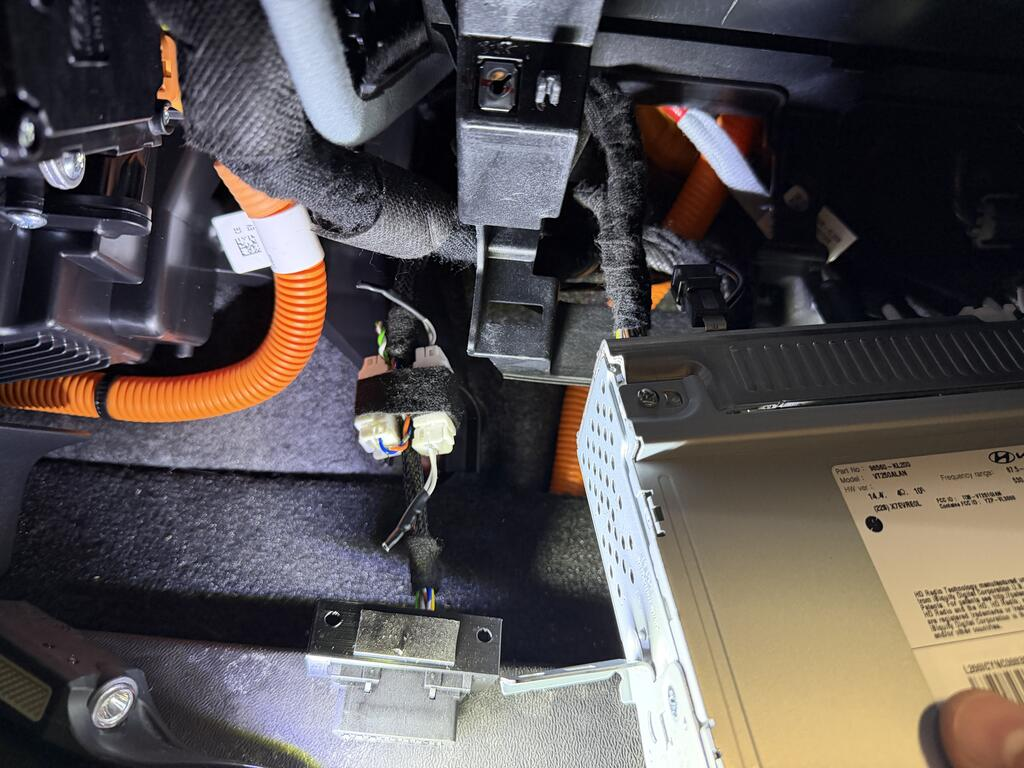
\includegraphics[height=1.5in,angle=0]{photos/harness_installed_HU_detached.jpg} }  
  \subfloat[]{\label{subfig:obd:installed}
  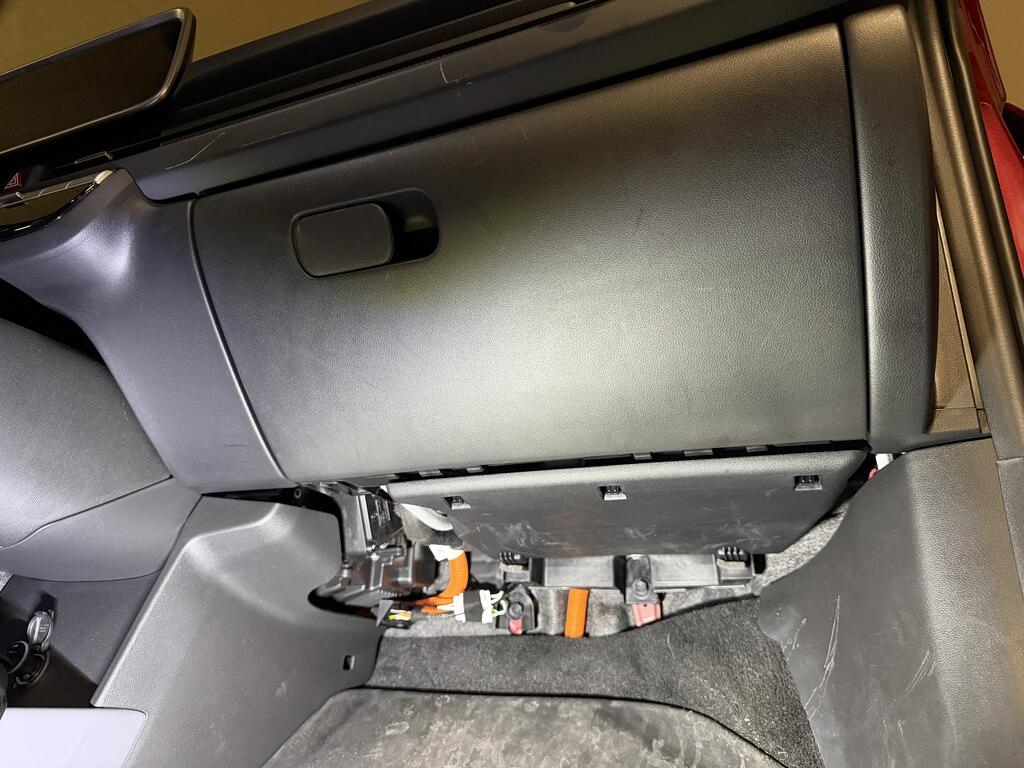
\includegraphics[height=1.5in,angle=0]{photos/harness_installed_1.jpg} } 
  \subfloat[]{\label{subfig:obd:wican}
  \includegraphics[height=1.5in,angle=0]{../Ioniq5/photos/wican_inserted.jpg} } 
   \caption{(a) OBD-Anschluss über die Halterung des Steuergeräts geschraubt. (b) Kabelbaum mit Kabelbindern an vorhandenem Kabel befestigt. (c) WiCAN-Anschluss in den OBD-Anschluss gesteckt. \label{fig:obd}}
\end{figure}

\section{Schritt 5: Aufräumen} \label{sect:4}
Führen Sie die Schritte zum Entfernen der Verkleidung in umgekehrter Reihenfolge aus. Achten Sie darauf, dass die Verkleidungsclips richtig ausgerichtet sind, und drücken Sie die Verkleidungsteile dann fest wieder ein. Schließen Sie den Minuspol der 12-V-Batterie wieder an. Das WiCAN-Gerät sollte sofort eine blaue LED anzeigen. Ändern Sie Ihr WiCAN-Passwort: \href{https://meatpihq.github.io/wican-fw/config/wifi}{https://meatpihq.github.io/wican-fw/config/wifi}Sie können Ihr WiCAN-Gerät direkt verbinden, indem Sie ein WLAN-Netzwerk mit dem Namen „WiCAN“ suchen.\_xxxxxxx' und geht zu \href{http://192.168.80.1/}{http://192.168.80.1/} in Ihrem Browser.
% \appendix 
\end{document}
